\chapter{L'architettura impossibile del cervello: 500 milioni di anni di improvvisazione}

\begin{flushright}
	\textit{``Siamo stati costruiti per sopravvivere, non per essere felici.''}\\[6pt]
	\textsc{Robert Wright}
\end{flushright}

\bigskip
\bigskip

\section{Il sabotatore nella testa}

Immaginate di trovarvi in una libreria. State sfogliando un volume che sembra promettente, quando notate il nome dell'autore sul frontespizio. \`{E} qualcuno che avete visto in tv, o forse sui social, anni fa. Vi aveva fatto una pessima impressione: arrogante, supponente, uno di quegli individui che riempiono ogni conversazione solo della propria voce. In quel preciso istante, senza che ve ne accorgiate minimamente, il vostro cervello ha gi\`{a} deciso. Il libro non vale la pena. Lo rimettete sullo scaffale e vi allontanate.

Cosa \`{e} appena successo? Un sistema neurologico progettato  centomila anni fa per valutare se un membro della trib\`{u} fosse affidabile o pericoloso ha appena giudicato un'opera intellettuale basandosi su un'interazione di cinque minuti avvenuta anni prima. \`{E} come se un algoritmo preistorico concepito per distinguere bacche velenose da quelle commestibili stesse ora decidendo cosa leggere, chi amare, come investire i vostri risparmi.

Questo \`{e} il paradosso della condizione umana moderna: navighiamo un mondo di idee astratte, mercati finanziari e relazioni digitali usando un cervello ottimizzato per sopravvivere nella savana africana. Dentro la vostra testa vive quello che potremmo chiamare un \textit{sabotatore cognitivo}. Non \`{e} cattivo, non ce l'ha con voi. \`{E} semplicemente un sistema operativo progettato per un mondo che non esiste pi\`{u}, che continua a prendere decisioni basandosi su un manuale scritto quando il problema pi\`{u} complesso era distinguere un ramo da un serpente.

C'\`{e} qualcosa di commovente in questa impotenza. E c'\`{e} anche qualcosa di antico, molto pi\`{u} antico di quanto potremmo immaginare. Gi\`{a} ventiquattro secoli prima che la neurologia nascesse come scienza, un filosofo ad Atene aveva intuito questo stesso conflitto con una chiarezza quasi soprannaturale. Platone, nel dialogo \textit{Fedro}, descrisse l'anima umana con un'immagine di tale potenza visiva da attraversare intatta millenni di storia del pensiero: un cocchiere che tenta di governare un carro tirato da due cavalli di natura radicalmente opposta.\footnote{Platone. \textit{Fedro}, 246a e seguenti. Traduzione di Giovanni Reale. Bompiani, Milano, 2000.}

Il primo cavallo \`{e} nobile, bianco, amante dell'onore e della bellezza, docile alla parola del cocchiere. Il secondo \`{e} nero, tozzo, impulsivo, sordo a ogni ragionamento, trascinato dall'istinto e dal desiderio. Il cocchiere, la ragione, deve tenere le redini di entrambi. Ma i cavalli sono enormi e lui \`{e} solo un uomo.

Quella è stata la prima grande mappa della mente divisa. E come vedremo, non sar\`{a} n\`{e} l'ultima n\`{e} la meno precisa.

\section{Origini di un capolavoro imperfetto: il costo di pensare}

Per capire davvero perch\`{e} il vostro cervello vi tradisce ogni volta che restate svegli fino all'una sapendo di dover essere operativi alle sette di mattina, dobbiamo fare un viaggio nel tempo. Un viaggio molto lungo.

Immaginate le acque torbide del periodo Cambriano, circa 500 milioni di anni fa. Qui nuotano creature che sembrano uscite da un incubo cosmico: \textit{Anomalocaris} con i suoi occhi composti giganteschi, \textit{Opabinia} con le sue cinque protuberanze oculari, \textit{Hallucigenia} che i paleontologi hanno ricostruito per decenni letteralmente sottosopra, convinti che le spine fossero zampe e viceversa.\footnote{Morris, S. C., e Caron, J. B. (2012). Pikaia gracilens Walcott, a stem-group chordate from the Middle Cambrian of British Columbia. \textit{Biological Reviews}, 87(2).}

\begin{center}
	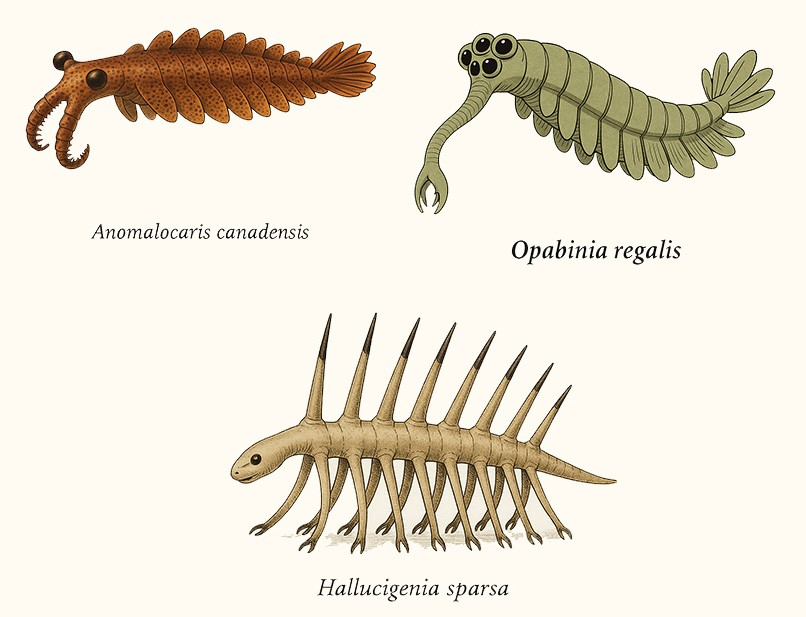
\includegraphics[width=0.75\textwidth]{images/cambriano_alieni.jpg}
	\captionof{figure}{Le bizzarre creature del Cambriano: Anomalocaris, Opabinia e Hallucigenia. Da questi esperimenti evolutivi emergeranno, in 500 milioni di anni di tentativi e improvvisazioni successive, i primi sistemi nervosi e infine il cervello umano.}
	\label{fig:cambriano_creature}
\end{center}

In questo teatro dell'assurdo evolutivo nasce la prima versione di quello che diventer\`{a} il nostro sistema nervoso. Non chiamatelo ancora cervello: \`{e} pi\`{u} simile a un interruttore biologico con due sole posizioni, ``mangia'' oppure ``scappa''. Eppure, in questa semplicità brutale c'\`{e} gi\`{a} il seme di tutti i nostri futuri problemi. Quel protoneurone che urlava ``pericolo!'' al minimo stimolo ambiguo \`{e} l'antenato diretto dello stesso sistema che oggi vi fa sobbalzare quando il tostapane espelle il pane troppo rumorosamente.

Ma c'\`{e} un problema che ha condizionato tutto, un vincolo fisico che l'evoluzione non ha mai potuto ignorare: \textit{pensare costa caro}.

Il cervello umano moderno \`{e} un paradosso metabolico. Rappresenta appena il due per cento del nostro peso corporeo, ma divora il venti per cento di tutta l'energia che consumiamo.\footnote{Raichle, M. E., e Gusnard, D. A. (2002). Appraising the brain's energy budget. \textit{Proceedings of the National Academy of Sciences}, 99(16).} \`{E} come avere una Ferrari nel garage che consuma benzina anche da ferma, anche mentre dorme, anche mentre guarda la televisione. In un mondo in cui le calorie erano scarse e preziose, ogni processo mentale doveva giustificare il proprio costo energetico.

Pensate a cosa significa nella pratica. I vostri antenati dovevano procurarsi circa duemila calorie al giorno per sopravvivere. Di queste, quattrocento se le consumava il cervello solo per esistere. Ogni volta che dovevano prendere una decisione complessa, analizzare davvero se quel rumore era vento o predatore, il consumo saliva ulteriormente. Ogni secondo di riflessione era un lusso che poteva costare la vita.

L'evoluzione ha trovato una soluzione tanto geniale quanto spietata: i \textit{bias cognitivi}. Invece di analizzare ogni situazione da zero, il cervello usa scorciatoie. Vede una forma allungata nell'erba? Serpente. Non importa se nel novantanove per cento dei casi \`{e} solo un ramo. Quella volta che \`{e} davvero un serpente, la scorciatoia salva la vita. Il costo di saltare per niente \`{e} minimo. Il costo di non saltare quando serve \`{e} fatale.

Non \`{e} stupidità. \`{E} ingegneria di sopravvivenza. Ma \`{e} la stessa ingegneria che oggi vi fa scegliere di non leggere un libro perch\`{e} l'autore vi era antipatico.

Fran\c{c}ois Jacob, premio Nobel per la medicina, descrisse l'evoluzione come un \textit{bricoleur}: un tuttofare che si arrangia sempre con quello che trova in garage, non come un ingegnere che progetta da zero su carta bianca.\footnote{Jacob, F. (1977). Evolution and tinkering. \textit{Science}, 196(4295).} L'evoluzione non pu\`{o} buttare via il vecchio cervello rettiliano e ricominciare da capo. Deve costruirci sopra, intorno, attraverso. Il risultato \`{e} inevitabilmente un pasticcio magnifico. Un'architettura mentale che sembra progettata da tre architetti separati da milioni di anni di storia, costretti a condividere sessanta centimetri cubi di spazio craniale e un solo budget energetico.

\section{Il carro alato e il condominio senza amministratore}

Paul MacLean, neuroscienziato al National Institute of Mental Health, negli anni Sessanta propose quello che chiam\`{o} il modello del ``cervello trino''.\footnote{MacLean, P. D. (1990). \textit{The Triune Brain in Evolution: Role in Paleocerebral Functions}. Plenum Press, New York.} MacLean non stava semplicemente descrivendo un'anatomia: stava raccontando la storia di come siamo diventati umani senza mai smettere di essere cavernicoli. La sua intuizione era questa: il cervello non \`{e} un organo unitario. \`{E} un edificio costruito su fondamenta antichissime, in cui ogni epoca geologica ha aggiunto un piano senza demolire quelli precedenti.

\begin{center}
	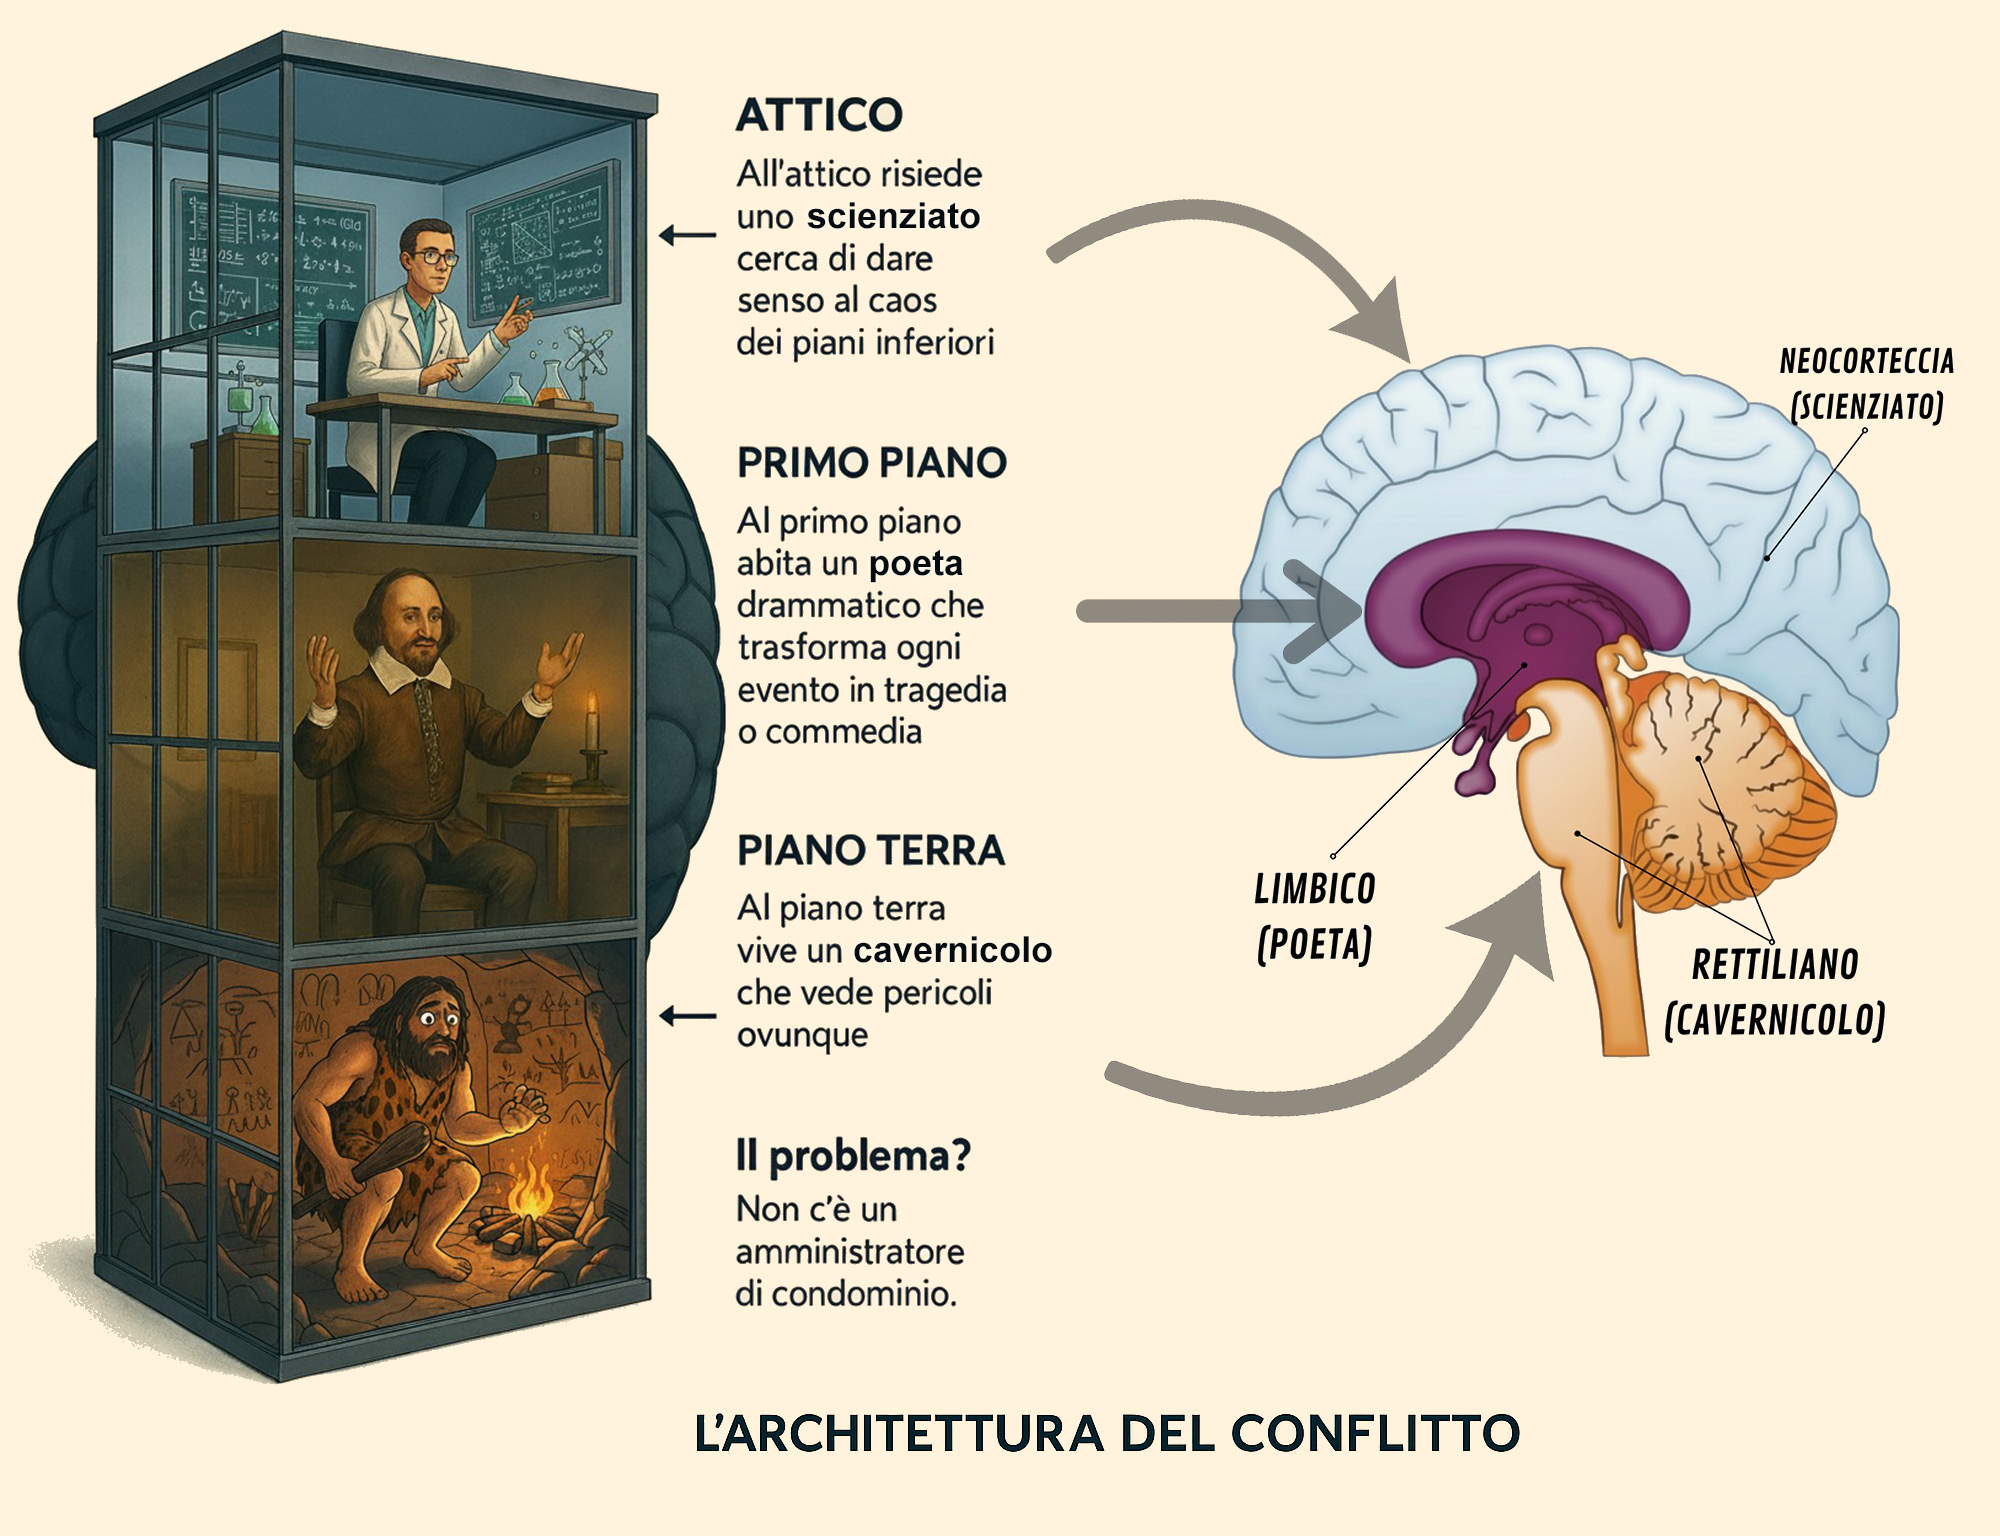
\includegraphics[width=1.0\textwidth]{images/bias_condominio3.jpg}
	\captionof{figure}{L'architettura del conflitto: tre inquilini che non si sono scelti ma sono costretti a convivere. Al piano terra il cavernicolo (cervello rettiliano), al primo piano il poeta drammatico (sistema limbico), all'attico lo scienziato razionale (neocorteccia). Non esiste un amministratore di condominio.}
	\label{fig:cervello_trino}
\end{center}

Osservate l'immagine. Al piano terra, accovacciato davanti a un fuoco immaginario, vive il \textit{cervello rettiliano}. \`{E} l\`{i} da 500 milioni di anni. Conosce solo pericoli immediati: predatori, fame, freddo, territorio. Per lui ogni ombra \`{e} una minaccia, ogni rumore sospetto \`{e} un segnale d'allarme. Controlla l'interruttore dell'adrenalina e quando decide che c'\`{e} pericolo (e quasi tutto \`{e} pericolo, nel suo vocabolario) inonda l'intero edificio di ormoni dello stress prima ancora che gli altri inquilini capiscano cosa sta succedendo.

Al primo piano abita un \textit{sistema limbico} shakespeariano, un poeta elisabettiano della neurologia che trasforma ogni stimolo in dramma esistenziale. Un collega che non saluta diventa tradimento personale. Un parcheggio rubato si trasforma in oltraggio all'onore. Un complimento del capo genera euforia da incoronazione regale, mentre una critica anche costruttiva precipita nell'abisso della tragedia greca. Non esistono mezze misure nel suo teatro interno.

Infine, nell'attico, circondato da lavagne piene di equazioni, lavora uno \textit{scienziato moderno}: la neocorteccia. Sa calcolare probabilit\`{a}, valutare rischi, pianificare strategie. Ha dimostrato matematicamente che rispondere alle email di lavoro dopo mezzanotte peggiora la qualit\`{a} delle decisioni del sessantadue per cento. Ma mentre lui perfeziona algoritmi decisionali, il cavernicolo del piano terra ha gi\`{a} suonato l'allarme e il poeta sta gi\`{a} riscrivendo l'intera storia come una tragedia greca.

Il problema fondamentale \`{e} che non c'\`{e} nessun amministratore di condominio. \`{E} un'anarchia neurologica dove il voto del cavernicolo che grida ``pericolo!'' vale quanto, spesso pi\`{u}, dell'analisi statistica dello scienziato.

A questo punto occorre fare una precisazione onesta. Negli ultimi anni il modello del cervello trino di MacLean \`{e} stato ampiamente criticato e in parte superato dalle neuroscienze moderne.\footnote{Cesario, J., Johnson, D. J., e Eisthen, H. L. (2020). Your brain is not an onion with a tiny reptile inside. \textit{Current Directions in Psychological Science}, 29(3).} Grazie alle tecnologie di neuroimmagine abbiamo scoperto che il cervello \`{e} una rete integrata di straordinaria complessit\`{a}, non un condominio a tre piani con inquilini separati. Le emozioni non abitano solo nel sistema limbico. La razionalit\`{a} non risiede solo nella neocorteccia. Tutto \`{e} molto pi\`{u} intrecciato, diffuso, interconnesso.

Eppure, e qui sta la cosa affascinante, come \textit{metafora} per capire cosa ci succede nella testa ogni giorno, il modello del cervello trino funziona ancora magnificamente. Non sar\`{a} anatomicamente preciso, ma descrive in modo perfetto quella sensazione di avere tre voci diverse che litigano tra loro. \`{E} un po' come le mappe della metropolitana: non rispettano le distanze reali n\`{e} la geografia della citt\`{a}, ma sono perfette per orientarsi.

Torniamo ora al carro alato di Platone. L'auriga che tenta di governare i due cavalli corrisponde esattamente alla nostra tripartizione neurologica. Il cavallo nobile e bianco (il \textit{thymos}, lo spirito, la volont\`{a} d'onore) risuona con il sistema limbico, quella sede delle emozioni sociali, dell'orgoglio e della vergogna. Il cavallo nero ribelle (l'\textit{epithymia}, il desiderio bruto, la pulsione immediata) corrisponde al cervello rettiliano, alla fame, alla paura, all'istinto di sopravvivenza. E il cocchiere razionale (il \textit{logos}) \`{e} la neocorteccia che tenta disperatamente di tenere le redini.\footnote{Platone. \textit{La Repubblica}, libro IV, 434d e seguenti. Traduzione di Mario Vegetti. BUR, Milano, 2007.}

Platone aveva disegnato la mappa. MacLean aveva scoperto il territorio. 

\begin{comment} % da mettere da qualche altra parte
\section{Il narratore che non capisce i numeri}

C'\`{e} un'altra conseguenza di questa architettura improvvisata che merita una riflessione a s\`{e}. Questo algoritmo ancestrale ha un punto cieco gigantesco: non capisce la statistica. E nel mondo moderno, dove quasi tutto funziona secondo logiche probabilistiche, questo \`{e} un problema serio.

Il nostro cervello \`{e} un \textit{narratore compulsivo} che trasforma automaticamente dati e coincidenze in storie coerenti, anche quando quelle storie non esistono. Il fenomeno \`{e} stato documentato in modo elegante dagli psicologi Timothy Wilson e Richard Nisbett in un esperimento ormai classico. Avevano allestito un banchetto con quattro paia di calze identiche, letteralmente identiche (stesso produttore, stesso lotto di produzione), disposte in fila da sinistra a destra. Chiedevano ai passanti di scegliere le calze di migliore qualit\`{a}. I risultati erano sistematici: le persone sceglievano quasi sempre le calze posizionate pi\`{u} a destra, per un semplice effetto della posizione. Ma la parte davvero interessante arrivava dopo. Quando i ricercatori domandavano perch\`{e} avessero scelto quelle calze, nessuno rispondeva ``perch\`{e} erano le pi\`{u} a destra''. Invece inventavano spiegazioni dettagliate e convincenti: ``La tessitura sembrava pi\`{u} fine'', ``Il colore era pi\`{u} brillante'', ``Si sentivano pi\`{u} morbide al tatto''. Stavano letteralmente fabbricando ragioni per giustificare una scelta inconscia basata sulla semplice posizione spaziale.\footnote{Nisbett, R. E., e Wilson, T. D. (1977). Telling more than we can know: Verbal reports on mental processes. \textit{Psychological Review}, 84(3).}

Questo meccanismo, che i neuropsicologi chiamano \textit{confabulazione}, \`{e} cos\`{i} automatico che non riusciamo nemmeno a percepirlo.\footnote{Hirstein, W. (2005). \textit{Brain Fiction: Self Deception and the Riddle of Confabulation}. MIT Press, Cambridge.} Non \`{e} un difetto caratteriale. \`{e} una caratteristica evolutiva fondamentale. Il nostro sistema nervoso non tollera vuoti narrativi. Quando mancano informazioni, il cervello le inventa istantaneamente, costruendo spiegazioni causali che ``tengano insieme'' gli eventi. \`{E} come un romanziere compulsivo che non sopporta trame con buchi nella logica. Per milioni di anni, questo istinto narrativo ci ha tenuti in vita: chi si fermava a verificare ogni dettaglio finiva spesso mangiato. Meglio una storia sbagliata ma veloce che un'analisi accurata ma tardiva.

Ancora pi\`{u} inquietante \`{e} il cosiddetto \textit{effetto cornice}. Un chirurgo che dice ``novanta per cento di possibilit\`{a} di successo'' ci tranquillizza. Se dice ``dieci per cento di possibilit\`{a} di morte'', probabilmente scappiamo dalla sua sala d'aspetto. Stessi numeri esatti, reazione radicalmente opposta.\footnote{Tversky, A., e Kahneman, D. (1981). The framing of decisions and the psychology of choice. \textit{Science}, 211(4481).} Il cavernicolo del piano terra sente la parola ``morte'' e attiva tutti gli allarmi, indipendentemente dalla matematica coinvolta. Lo scienziato nell'attico non riesce nemmeno ad aprire bocca.

La scoperta pi\`{u} sorprendente \`{e} che questo stesso meccanismo di costruzione narrativa \`{e} emerso nelle intelligenze artificiali. Le ``allucinazioni'' dell'intelligenza artificiale non sono errori tecnici nel senso tradizionale del termine: sono il modo in cui anche i sistemi artificiali riempiono i vuoti informativi con storie plausibili. \`{E} come se la tendenza a confabulare fosse intrinseca a qualsiasi sistema che debba processare informazioni incomplete in tempo reale. La natura e la tecnologia, per strade completamente diverse, hanno trovato la stessa soluzione imperfetta allo stesso problema.

Viviamo nell'epoca con pi\`{u} dati statistici di qualsiasi generazione nella storia umana, eppure prendiamo spesso decisioni peggiori dei nostri bisnonni che disponevano di informazioni frammentarie. Il paradosso non \`{e} l'eccesso di dati: \`{e} avere un sistema operativo progettato per processare al massimo una manciata di variabili contemporaneamente.

\end{comment}
\section{Tre mappe per la stessa anima divisa}

Duemilaquattrocento anni separano Platone da MacLean, eppure i due arrivano alla stessa conclusione: dentro di noi convivono forze che non condividono né il linguaggio né gli obiettivi. E non sono i soli ad averlo intuito.

Platone, con il suo carro alato, fu il primo a tracciare questa mappa: la vita felice, per lui, non era quella in cui il cocchiere soffoca i cavalli, ma quella in cui riesce a governarli entrambi.

Nel 1923, Sigmund Freud pubblic\`{o} \textit{Das Ich und das Es} (L'Io e l'Es), introducendo la sua tripartizione dell'apparato psichico: l'Es (sede degli istinti pi\`{u} primitivi, della pulsione di piacere e di morte), l'Io (il mediatore che tenta di tenere insieme le esigenze della realt\`{a}) e il Super io (la voce normativa interiorizzata della cultura e dei genitori).\footnote{Freud, S. (1923). \textit{Das Ich und das Es}. Internationaler Psychoanalytischer Verlag, Leipzig.} Il ``sabotatore cognitivo'' di cui abbiamo parlato all'inizio di questo capitolo corrisponde esattamente all'Es freudiano: la parte pi\`{u} antica, automatica e impulsiva della nostra mente, quella che agisce prima ancora che l'Io abbia avuto il tempo di rendersi conto che stava succedendo qualcosa.

Negli anni Sessanta, Paul MacLean traccia la mappa anatomica che già conosciamo: cervello rettiliano, sistema limbico, neocorteccia. Tre nomi nuovi per gli stessi inquilini.

E nel 2011, il Nobel Daniel Kahneman sintetizza l'intera tradizione in un'elegante semplificazione: il \textit{Sistema 1} (veloce, automatico, emotivo, ancestrale) e il \textit{Sistema 2} (lento, deliberato, razionale, costoso energeticamente).\footnote{Kahneman, D. (2011). \textit{Thinking, Fast and Slow}. Farrar, Straus and Giroux, New York.} Le tre forze di un tempo si riducono, con Kahneman, a due soli sistemi, per descrivere lo stesso conflitto fondamentale: la velocit\`{a} istintiva contro la lentezza riflessiva.

Quattro pensatori, quattro epoche storiche, quattro vocabolari completamente diversi. La stessa mappa.

\begin{figure}[htbp]
	\centering
	\includegraphics[width=0.80\textwidth]{images/tre_mappe_anima.png}
	\caption{Tre mappe per la stessa anima divisa. La tripartizione platonica (logos, thymos, epithymia), il modello freudiano (Io, Es, Super-io) e il cervello trino di MacLean descrivono, con linguaggi diversi e a distanza di secoli, la stessa architettura conflittuale della mente umana. Kahneman la sintetizza nel contrasto tra Sistema 1 e Sistema 2.}
	\label{fig:tre_mappe}
\end{figure}

Ma c'\`{e} un altro pensatore che ha intuito tutto questo nel modo forse pi\`{u} sorprendente di tutti, e dal posto pi\`{u} inaspettato: una mente matematica.

Blaise Pascal era un prodigio. A diciotto anni aveva costruito una delle prime calcolatrici meccaniche della storia. Aveva contribuito alla nascita del calcolo delle probabilit\`{a}. Aveva dimostrato teoremi di geometria proiettiva che ancora oggi portano il suo nome. Era, in breve, uno degli intelletti pi\`{u} rigorosi del XVII secolo. Eppure, nelle sue note personali pubblicate postume con il titolo di \textit{Pens\'{e}es}, scrisse una delle frasi pi\`{u} antiscientifiche che si possano immaginare uscite dalla penna di uno scienziato: ``Il cuore ha ragioni che la ragione non conosce''.\footnote{Pascal, B. (1670). \textit{Pens\'{e}es}. Pubblicazione postuma, Parigi.}

Un genio del calcolo che ammetteva i limiti del calcolo. Un maestro della logica che riconosceva una logica diversa, una logica del cuore che precede e supera la logica della dimostrazione.

Quella ``logica del cuore'' \`{e} esattamente ci\`{o} che oggi chiamiamo Sistema 1. \`{E} la velocit\`{a} ancestrale delle scorciatoie cognitive. \`{E} il cavernicolo del piano terra che ha gi\`{a} deciso prima che lo scienziato dell'attico abbia terminato di raccogliere le prove. Pascal non aveva le neuroscienze, non aveva le TAC funzionali, non aveva Kahneman. Ma aveva capito la cosa essenziale: esistono due modi di conoscere, e quello pi\`{u} rapido non passa per la ragione.

E qua la domanda chiave. Se il nostro Sistema 1 prende la maggior parte delle decisioni prima che il Sistema 2 abbia avuto tempo di intervenire; se il cavernicolo ha l'accesso diretto al sistema di allarme e pu\`{o} inondare l'intero edificio di adrenalina in pochi millisecondi; se l'attività cerebrale che precede un nostro gesto volontario si accende un istante prima che ne diventiamo consapevoli... siamo davvero noi ad agire? \textit{O siamo soltanto esseri razionali che scrivono le memorie di decisioni già prese da qualcun altro?}

La risposta onesta \`{e} che non lo sappiamo con certezza. Ma la domanda stessa \`{e} preziosa. Perch\`{e} nel momento in cui vi accorgete che il vostro Sistema 1 stava gi\`{a} rimettendo il libro sullo scaffale, qualcosa di importante \`{e} successo: il Sistema 2 si \`{e} svegliato. La consapevolezza dell'automatismo \`{e} gi\`{a}, in qualche misura, la sua prima incrinatura.

Non ne uscirete ``guariti'', non c'\`{e} niente da cui guarire. Il sabotatore cognitivo continuer\`{a} a fare il suo lavoro perch\`{e} \`{e} questo il suo scopo evolutivo, e per centinaia di migliaia di anni lo ha fatto magnificamente. Ma \`{e} come quando qualcuno vi fa notare che state respirando: all'improvviso ne diventate consapevoli, e per un attimo potete scegliere come farlo.

Questo libro vuole fare la stessa cosa con i vostri pensieri.

La strada prosegue. Perch\`{e} se il cervello trino ci ha mostrato l'architettura del conflitto, esiste un inquilino del condominio che merita un'attenzione particolare, uno che ha le chiavi di tutte le porte e le usa con una frequenza imbarazzante nel mondo contemporaneo. \`{E} il sistema pi\`{u} antico, pi\`{u} veloce e pi\`{u} potente che abbiamo. \`{E} il sistema che un leopardo nella savana aveva selezionato con una pressione evolutiva di decine di milioni di anni, e che oggi scatta per un messaggio visualizzato senza risposta.

\`{E} la paura. Ed \`{e} l\`{i} che andremo nel prossimo capitolo.